\documentclass[conference]{IEEEtran}
\IEEEoverridecommandlockouts
\usepackage[utf8]{inputenc}
\usepackage[T1]{fontenc}
\usepackage{cite}
\usepackage{amsmath,amssymb,amsfonts}
\usepackage{algorithmic}
\usepackage{graphicx}
\usepackage{textcomp}
\usepackage{xcolor}
\usepackage{booktabs}
\usepackage{multirow}
\usepackage[caption=false,font=footnotesize]{subfig}
\usepackage{hyperref}
\usepackage{array}
\graphicspath{{figs/}}
\hbadness=10000
\vbadness=10000
\def\BibTeX{{\rm B\kern-.05em{\sc i\kern-.025em b}\kern-.08em
    T\kern-.1667em\lower.7ex\hbox{E}\kern-.125emX}}

\begin{document}

\title{Flujo Completo de Structure from Motion para la Reconstrucci\'on 3D de Escenarios a partir de M\'ultiples Im\'agenes}

\author{\IEEEauthorblockN{Gustavo Perla, Juan Chicaiza, Santiago Reategui y Jorge Gomez}
\IEEEauthorblockA{\textit{Universidad San Francisco de Quito} \\
\textit{MAC5001 Visi\'on por Computadora}\\
}}

\maketitle

\begin{abstract}
Este trabajo presenta un flujo completo de \emph{Structure from Motion} (SfM) para la reconstrucci\'on 3D de objetos a partir de m\'ultiples im\'agenes capturadas por el equipo. A diferencia de un ejemplo aislado de alineamiento entre dos vistas, el proyecto integra preparaci\'on del dataset, extracci\'on y emparejamiento de caracter\'isticas, reconstrucci\'on incremental con COLMAP, limpieza del modelo disperso, an\'alisis del grafo de vistas, estudio de crecimiento por subconjuntos de im\'agenes y detecci\'on deliberada del efecto \emph{doppelganger}. El pipeline se evalu\'o sobre tres escenas reales: \emph{buda}, \emph{estatua} y \emph{leon}, con 521, 763 y 729 fotograf\'ias respectivamente. Los resultados muestran reconstrucciones finales robustas, con razones de registro de 1.00 para \emph{buda} y \emph{leon}, y 0.957 para \emph{estatua}; adem\'as, el filtrado geom\'etrico mejora la interpretabilidad visual del modelo al reducir puntos espurios. Como apoyo a la presentaci\'on del proceso, se construy\'o un notebook de visualizaci\'on que resume cada fase de la metodolog\'ia sin sacrificar la reproducibilidad del pipeline principal.
\end{abstract}

\begin{IEEEkeywords}
Structure from Motion, COLMAP, reconstrucci\'on 3D, grafo de vistas, reproyecci\'on, doppelganger, filtrado de nube dispersa
\end{IEEEkeywords}

\section{Introducci\'on}\label{sec:intro}

La reconstrucci\'on 3D a partir de m\'ultiples vistas es uno de los problemas fundamentales de la visi\'on por computadora. Dentro de este contexto, \emph{Structure from Motion} (SfM) permite estimar simult\'aneamente la geometr\'ia de la escena y las poses de c\'amara usando correspondencias visuales entre im\'agenes~\cite{b1,b2}. Este tipo de pipeline es relevante en fotogrametr\'ia, patrimonio cultural, rob\'otica, realidad aumentada y levantamiento digital de objetos.

La consigna original del proyecto solicit\'o evidenciar el flujo completo de SfM mediante un script Python o notebook, usando datasets propios, presentando la metodolog\'ia por fases, mostrando el crecimiento incremental de la reconstrucci\'on y forzando a prop\'osito el efecto \emph{doppelganger}. Sin embargo, durante la implementaci\'on del proyecto se evolucion\'o hacia un pipeline reproducible basado en \emph{scripts}, interfaz de l\'inea de comandos y contenedores Docker, con COLMAP como backend principal~\cite{b2,b3}. Esta decisi\'on facilit\'o la ejecuci\'on robusta sobre cientos de im\'agenes, pero alej\'o parcialmente el entregable del formato acad\'emico inicialmente pedido.

Por ello, el aporte de este trabajo es doble:
\begin{enumerate}
  \item consolidar el pipeline operativo completo que genera reconstrucciones reproducibles sobre tres datasets reales;
  \item reorganizar sus resultados en un flujo did\'actico y documentado, apoyado por un notebook de visualizaci\'on y por el presente informe en formato IEEE.
\end{enumerate}

Las escenas analizadas son tres objetos reales capturados por el equipo: \emph{buda}, \emph{estatua} y \emph{leon}. Sobre ellas se reportan estad\'isticas de registro, densidad de puntos 3D, error de reproyecci\'on, conectividad del grafo de vistas y candidatos \emph{doppelganger}. De esta manera, el trabajo pasa de ser solamente un entorno de ejecuci\'on a convertirse tambi\'en en un entregable acad\'emico alineado con la consigna original.

\section{Marco Metodol\'ogico}\label{sec:math}

\subsection{Flujo general de SfM}

El pipeline empleado sigue la metodolog\'ia cl\'asica de SfM:
\begin{enumerate}
  \item captura de im\'agenes con solapamiento suficiente alrededor del objeto;
  \item extracci\'on de caracter\'isticas locales SIFT sobre cada imagen;
  \item emparejamiento entre vistas usando estrategias \emph{sequential} o \emph{exhaustive};
  \item verificaci\'on geom\'etrica de pares y construcci\'on del grafo de vistas;
  \item reconstrucci\'on dispersa incremental para recuperar poses y puntos 3D;
  \item exportaci\'on del modelo textual para an\'alisis externo;
  \item filtrado no destructivo del modelo para mejorar su limpieza visual;
  \item an\'alisis incremental por subconjuntos de im\'agenes y detecci\'on de \emph{doppelgangers}.
\end{enumerate}

COLMAP implementa este flujo con detectores y descriptores robustos, emparejamiento geom\'etrico y un mapeador incremental ampliamente usado en investigaci\'on y aplicaciones reales~\cite{b2,b3}. En este proyecto, COLMAP se us\'o como motor de reconstrucci\'on, mientras que el c\'odigo propio se encarg\'o de la orquestaci\'on, an\'alisis posterior y visualizaci\'on.

\subsection{Grafo de vistas}

Una forma \'util de entender una reconstrucci\'on SfM es verla como un grafo \(G=(V,E)\), donde cada nodo representa una imagen y cada arista representa una relaci\'on geom\'etricamente consistente entre dos vistas. Si \(m_{ij}\) es el n\'umero de matches visuales entre las im\'agenes \(i\) y \(j\), y \(g_{ij}\) es el n\'umero de inliers geom\'etricos tras verificaci\'on, entonces el cociente
\begin{equation}
r_{ij} = \frac{g_{ij}}{m_{ij}}
\end{equation}
se usa como una medida de consistencia geom\'etrica. En este trabajo, dicho valor se emplea para ponderar la visualizaci\'on del grafo y estudiar su conectividad.

\subsection{M\'etricas de reconstrucci\'on}

Para medir la calidad de una reconstrucci\'on se usaron cuatro indicadores principales:
\begin{itemize}
  \item \textbf{im\'agenes registradas}: n\'umero de c\'amaras cuya pose fue estimada;
  \item \textbf{raz\'on de registro}: fracci\'on entre im\'agenes registradas e im\'agenes de entrada;
  \item \textbf{n\'umero de puntos 3D}: cardinalidad de la nube dispersa reconstruida;
  \item \textbf{error medio de reproyecci\'on}: promedio del error reportado por COLMAP sobre cada punto 3D.
\end{itemize}

Adicionalmente se reporta la longitud media de \emph{track}, es decir, el promedio de vistas que observan un mismo punto 3D. Un \emph{track} largo suele indicar una reconstrucci\'on m\'as estable.

\subsection{Efecto \emph{Doppelganger}}

En el contexto de este proyecto, un par \emph{doppelganger} es un par de im\'agenes que parecen altamente compatibles a nivel visual, pero cuya consistencia geom\'etrica relativa no es suficientemente fuerte. Para detectarlos se ejecut\'o un emparejamiento exhaustivo auxiliar sobre una copia separada de la base de COLMAP y se definieron pares sospechosos como aquellos con:
\begin{itemize}
  \item un n\'umero alto de coincidencias visuales crudas;
  \item una relaci\'on de inliers geom\'etricos menor o igual al umbral configurado.
\end{itemize}

En el pipeline se usa la puntuaci\'on
\begin{equation}
s_{ij} = m_{ij}(1-r_{ij}),
\end{equation}
donde valores grandes indican muchos matches visuales pero acuerdo geom\'etrico imperfecto. Este mecanismo satisface la parte del enunciado que pide inducir y documentar el efecto \emph{doppelganger}.

\section{Implementaci\'on}\label{sec:impl}

El proyecto se implement\'o en Python 3 y se organiz\'o como un paquete reutilizable llamado \texttt{sfm\_pipeline}. El backend de reconstrucci\'on es COLMAP y el resto de la l\'ogica se distribuye en comandos de l\'inea de comandos:

\begin{itemize}
  \item \texttt{prepare}: valida el dataset y genera el manifiesto de im\'agenes;
  \item \texttt{extract-match}: ejecuta extracci\'on de SIFT y matching en la base de COLMAP;
  \item \texttt{reconstruct}: corre el mapeador incremental y exporta el modelo textual;
  \item \texttt{clean-model}: filtra la nube dispersa exportada para remover puntos espurios;
  \item \texttt{analyze-graph}: construye el grafo de vistas y lo exporta a CSV, DOT y HTML;
  \item \texttt{detect-doppelgangers}: identifica pares visualmente ambiguos;
  \item \texttt{run-ablation}: ejecuta reconstrucciones sobre subconjuntos de tama\~no creciente;
  \item \texttt{report}: exporta gr\'aficas de las m\'etricas incrementales.
\end{itemize}

La estructura del proyecto se apoya tambi\'en en Docker, lo que permite ejecutar el mismo flujo tanto localmente como en GPU remota. Esta capa operativa es importante para reproducibilidad, pero para cumplir de mejor manera la consigna se agreg\'o un notebook de visualizaci\'on \texttt{notebooks/sfm\_visual\_workflow.ipynb}, que resume el pipeline por fases usando los artefactos ya generados.

\section{Datasets y Dise\~no Experimental}\label{sec:exp}

\subsection{Datasets}

Se trabaj\'o con tres conjuntos de im\'agenes creados por el equipo:
\begin{itemize}
  \item \textbf{buda}: 521 im\'agenes;
  \item \textbf{estatua}: 763 im\'agenes;
  \item \textbf{leon}: 729 im\'agenes.
\end{itemize}

Las capturas se realizaron rodeando cada objeto con solapamiento suficiente entre vistas consecutivas. En los tres casos se busc\'o un recorrido aproximadamente circular y distancia relativamente estable al objeto, aunque \emph{estatua} mostr\'o mayor dificultad por oclusiones, cambios de fondo y menor consistencia global.

\begin{figure*}[htbp]
  \centering
  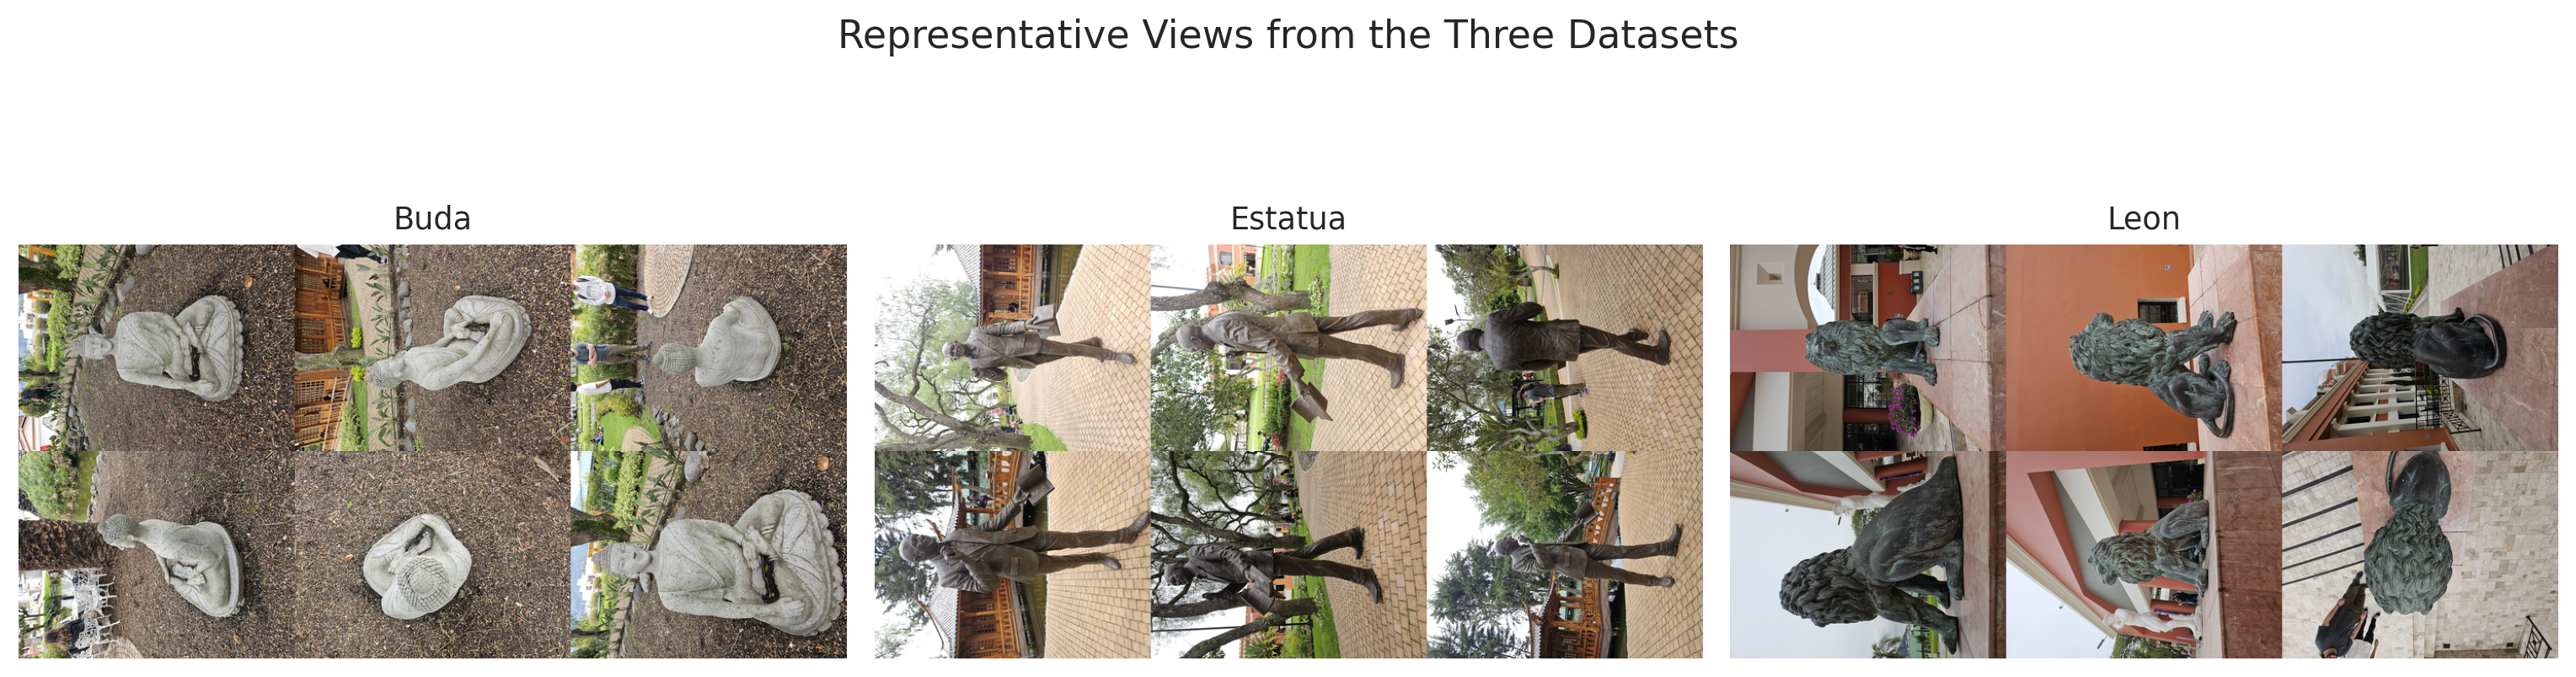
\includegraphics[width=0.95\textwidth]{dataset_samples.png}
  \caption{Muestras representativas de los tres datasets empleados en el proyecto.}
  \label{fig:dataset_samples}
\end{figure*}

\subsection{Configuraci\'on del pipeline}

El archivo de configuraci\'on principal usa:
\begin{itemize}
  \item modelo de c\'amara \texttt{SIMPLE\_RADIAL};
  \item \texttt{sequential\_matcher} como estrategia principal de matching;
  \item resoluci\'on m\'axima de 1200 px para la configuraci\'on base;
  \item hasta 4096 caracter\'isticas SIFT por imagen;
  \item solapamiento secuencial de 10 vecinos;
  \item umbral m\'inimo de 15 matches para el mapeador.
\end{itemize}

Para estudiar el crecimiento incremental de la reconstrucci\'on se ejecutaron ablaciones con subconjuntos aleatorios de tama\~no variable. En \emph{buda} se consideraron 20, 40 y 80 im\'agenes, mientras que en \emph{estatua} y \emph{leon} se extendi\'o el an\'alisis hasta 160 y 320 im\'agenes.

\section{Resultados}\label{sec:results}

\subsection{Resumen global}

La Tabla~\ref{tab:summary} resume el comportamiento final del pipeline completo. \emph{Buda} y \emph{leon} alcanzan registro total, mientras que \emph{estatua} presenta la escena m\'as desafiante con 730 de 763 im\'agenes registradas. Aun as\'i, su modelo final sigue siendo utilizable y denso.

\begin{table*}[htbp]
\caption{Resumen global de las reconstrucciones finales.}
\label{tab:summary}
\centering
\small
\begin{tabular}{lrrrrrrrr}
\toprule
\textbf{Objeto} & \textbf{Imgs.} & \textbf{Reg.} & \textbf{Ratio} & \textbf{Pts. brutos} & \textbf{Pts. filtrados} & \textbf{Err. bruto} & \textbf{Err. filtrado} & \textbf{Track prom.} \\
\midrule
\textbf{Buda}    & 521 & 521 & 1.000 & 188\,203 & 65\,825 & 1.406 & 1.343 & 19.213 \\
\textbf{Estatua} & 763 & 730 & 0.957 & 122\,140 & 27\,973 & 1.351 & 1.330 & 18.545 \\
\textbf{Leon}    & 729 & 729 & 1.000 & 157\,284 & 99\,122 & 1.236 & 1.138 & 25.655 \\
\bottomrule
\end{tabular}
\end{table*}

El filtrado reduce significativamente la cantidad de puntos para privilegiar la estructura principal del objeto. La reducci\'on es del \(65.0\%\) en \emph{buda}, \(77.1\%\) en \emph{estatua} y \(37.0\%\) en \emph{leon}. En los tres casos el error medio de reproyecci\'on mejora ligeramente, lo que indica que la limpieza no solo simplifica la visualizaci\'on sino que tambi\'en elimina puntos menos confiables.

\subsection{Conectividad entre vistas}

La Fig.~\ref{fig:view_graphs} muestra los grafos de conectividad para las tres escenas. El comportamiento es coherente con el proceso de captura: aparecen estructuras densas y fuertemente conectadas por proximidad temporal. Las estad\'isticas agregadas del grafo son:
\begin{itemize}
  \item \textbf{buda}: 3842 aristas, \emph{inlier ratio} medio de 0.969 y 4368.6 inliers por arista en promedio;
  \item \textbf{estatua}: 5358 aristas, \emph{inlier ratio} medio de 0.907 y 3630.0 inliers por arista;
  \item \textbf{leon}: 5261 aristas, \emph{inlier ratio} medio de 0.956 y 4369.9 inliers por arista.
\end{itemize}

La menor consistencia geom\'etrica de \emph{estatua} es consistente con su menor tasa de registro final.

\begin{figure*}[htbp]
  \centering
  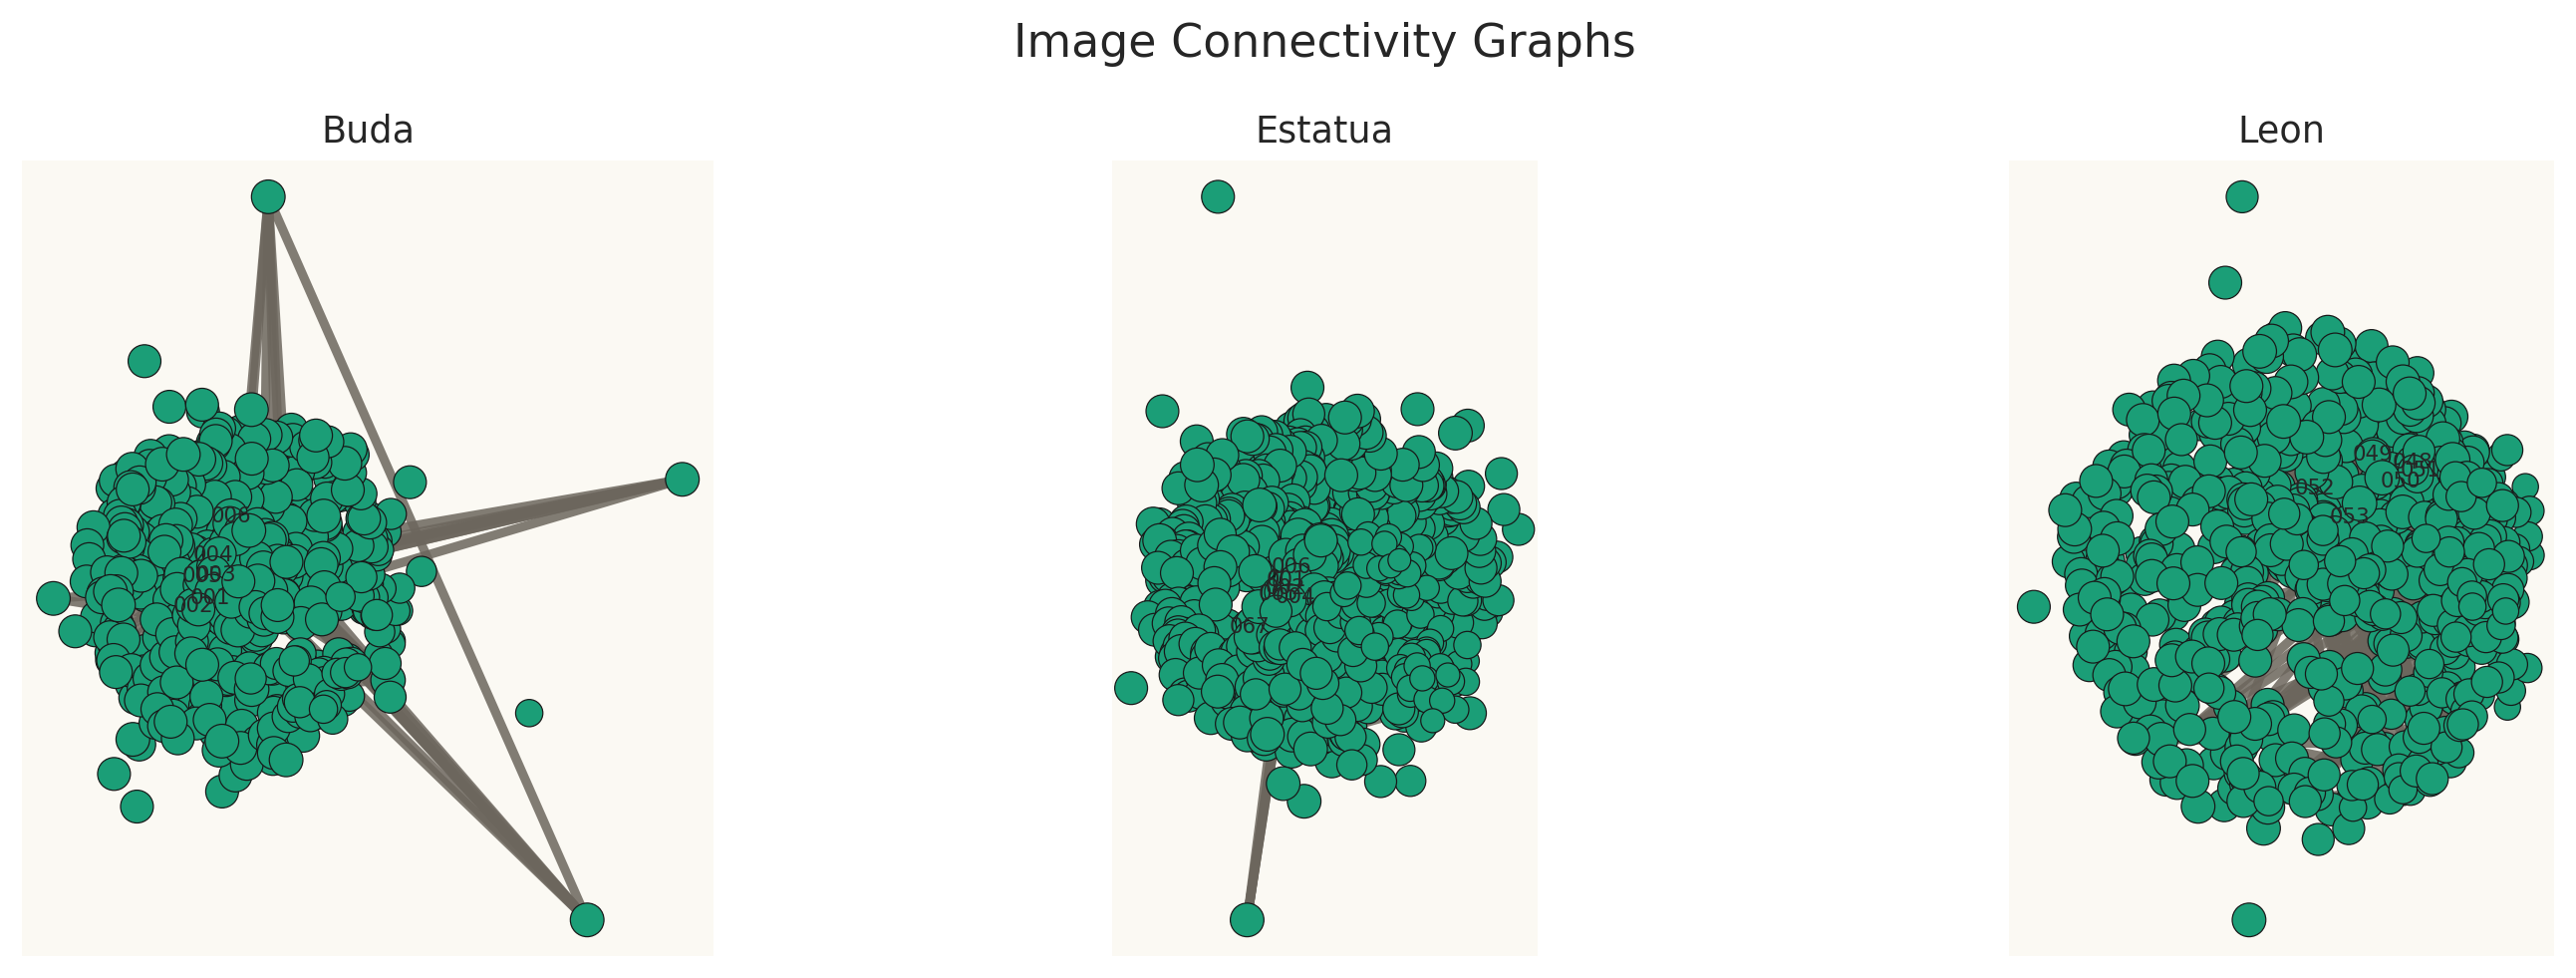
\includegraphics[width=0.95\textwidth]{view_graphs.png}
  \caption{Grafos de conectividad entre vistas. Los nodos representan im\'agenes y las aristas relaciones geom\'etricas v\'alidas.}
  \label{fig:view_graphs}
\end{figure*}

\subsection{Reconstrucci\'on incremental}

Una de las partes m\'as importantes de la consigna fue mostrar la reconstrucci\'on a medida que aumentan las vistas. La Fig.~\ref{fig:incremental} resume este comportamiento usando las corridas de ablaci\'on. Se observa una tendencia clara:
\begin{itemize}
  \item al aumentar el n\'umero de im\'agenes, crece el n\'umero de puntos 3D;
  \item la raz\'on de registro mejora marcadamente en \emph{estatua} y \emph{leon};
  \item el error de reproyecci\'on se mantiene relativamente estable, lo que sugiere que el incremento de densidad no sacrifica coherencia geom\'etrica.
\end{itemize}

La Tabla~\ref{tab:ablation} resume los promedios por tama\~no de subconjunto. \emph{Buda} es el objeto m\'as estable: incluso con 20 im\'agenes logra registro completo. \emph{Estatua} requiere un mayor n\'umero de vistas para estabilizarse, mientras que \emph{leon} muestra una mejora abrupta a partir de 80 im\'agenes.

\begin{figure*}[htbp]
  \centering
  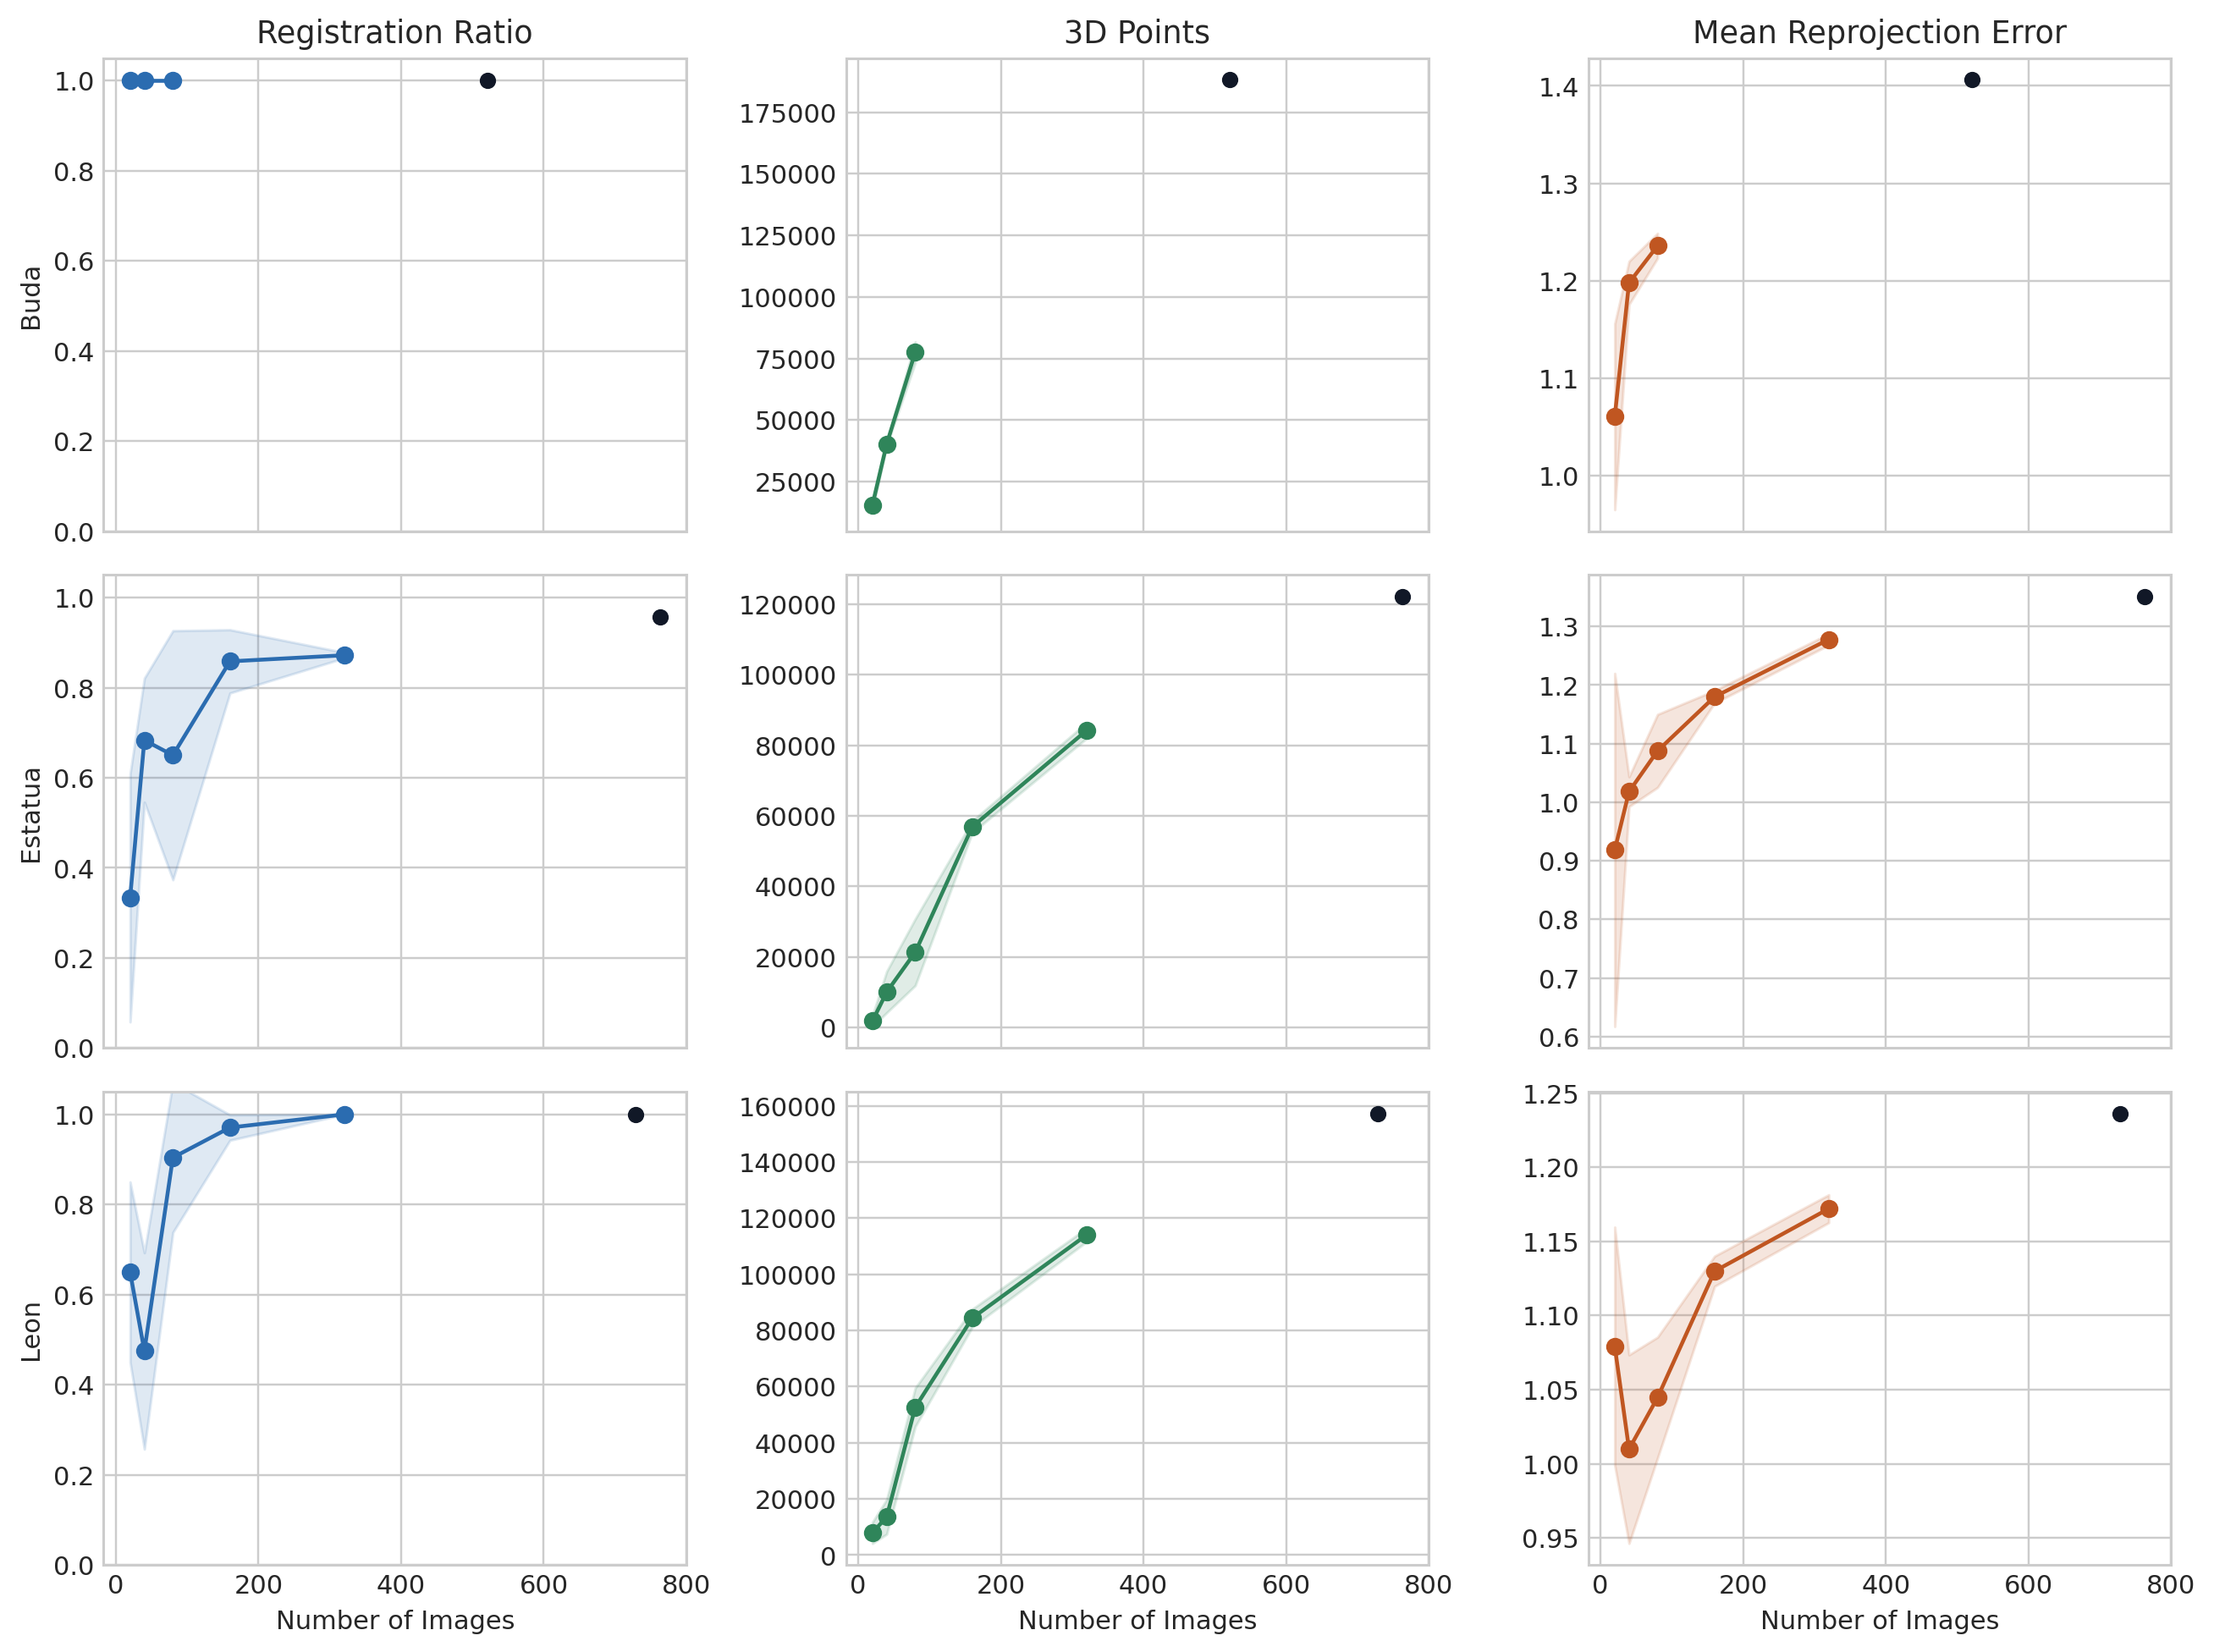
\includegraphics[width=0.92\textwidth]{incremental_metrics.png}
  \caption{Evoluci\'on incremental de la reconstrucci\'on al aumentar el n\'umero de im\'agenes.}
  \label{fig:incremental}
\end{figure*}

\begin{table*}[htbp]
\caption{Resultados promedio de ablaci\'on por n\'umero de im\'agenes.}
\label{tab:ablation}
\centering
\small
\begin{tabular}{llrrrr}
\toprule
\textbf{Objeto} & \textbf{Imgs.} & \textbf{Corridas} & \textbf{Ratio de registro} & \textbf{Puntos 3D promedio} & \textbf{Error medio} \\
\midrule
\multirow{3}{*}{Buda}
  & 20  & 3 & 1.0000 & 15\,505.0 & 1.0604 \\
  & 40  & 3 & 1.0000 & 40\,288.3 & 1.1977 \\
  & 80  & 3 & 1.0000 & 77\,507.7 & 1.2358 \\
\midrule
\multirow{5}{*}{Estatua}
  & 20  & 3 & 0.3333 & 1\,825.0  & 0.9185 \\
  & 40  & 3 & 0.6833 & 10\,054.7 & 1.0180 \\
  & 80  & 3 & 0.6500 & 21\,330.7 & 1.0876 \\
  & 160 & 3 & 0.8583 & 56\,884.3 & 1.1799 \\
  & 320 & 3 & 0.8719 & 84\,140.7 & 1.2777 \\
\midrule
\multirow{5}{*}{Leon}
  & 20  & 3 & 0.6500 & 7\,914.0   & 1.0792 \\
  & 40  & 3 & 0.4750 & 13\,604.0  & 1.0098 \\
  & 80  & 3 & 0.9042 & 52\,617.3  & 1.0446 \\
  & 160 & 3 & 0.9708 & 84\,394.7  & 1.1299 \\
  & 320 & 2 & 1.0000 & 113\,933.5 & 1.1720 \\
\bottomrule
\end{tabular}
\end{table*}

\subsection{Visualizaci\'on de modelos filtrados}

La Fig.~\ref{fig:pointclouds} muestra las nubes dispersas filtradas. Aunque se trata todav\'ia de modelos dispersos, se distinguen claramente las formas principales de los tres objetos. \emph{Leon} presenta la nube m\'as estable y con mayor soporte multi-vista, lo cual tambi\'en se refleja en su longitud media de \emph{track} de 25.655.

\begin{figure*}[htbp]
  \centering
  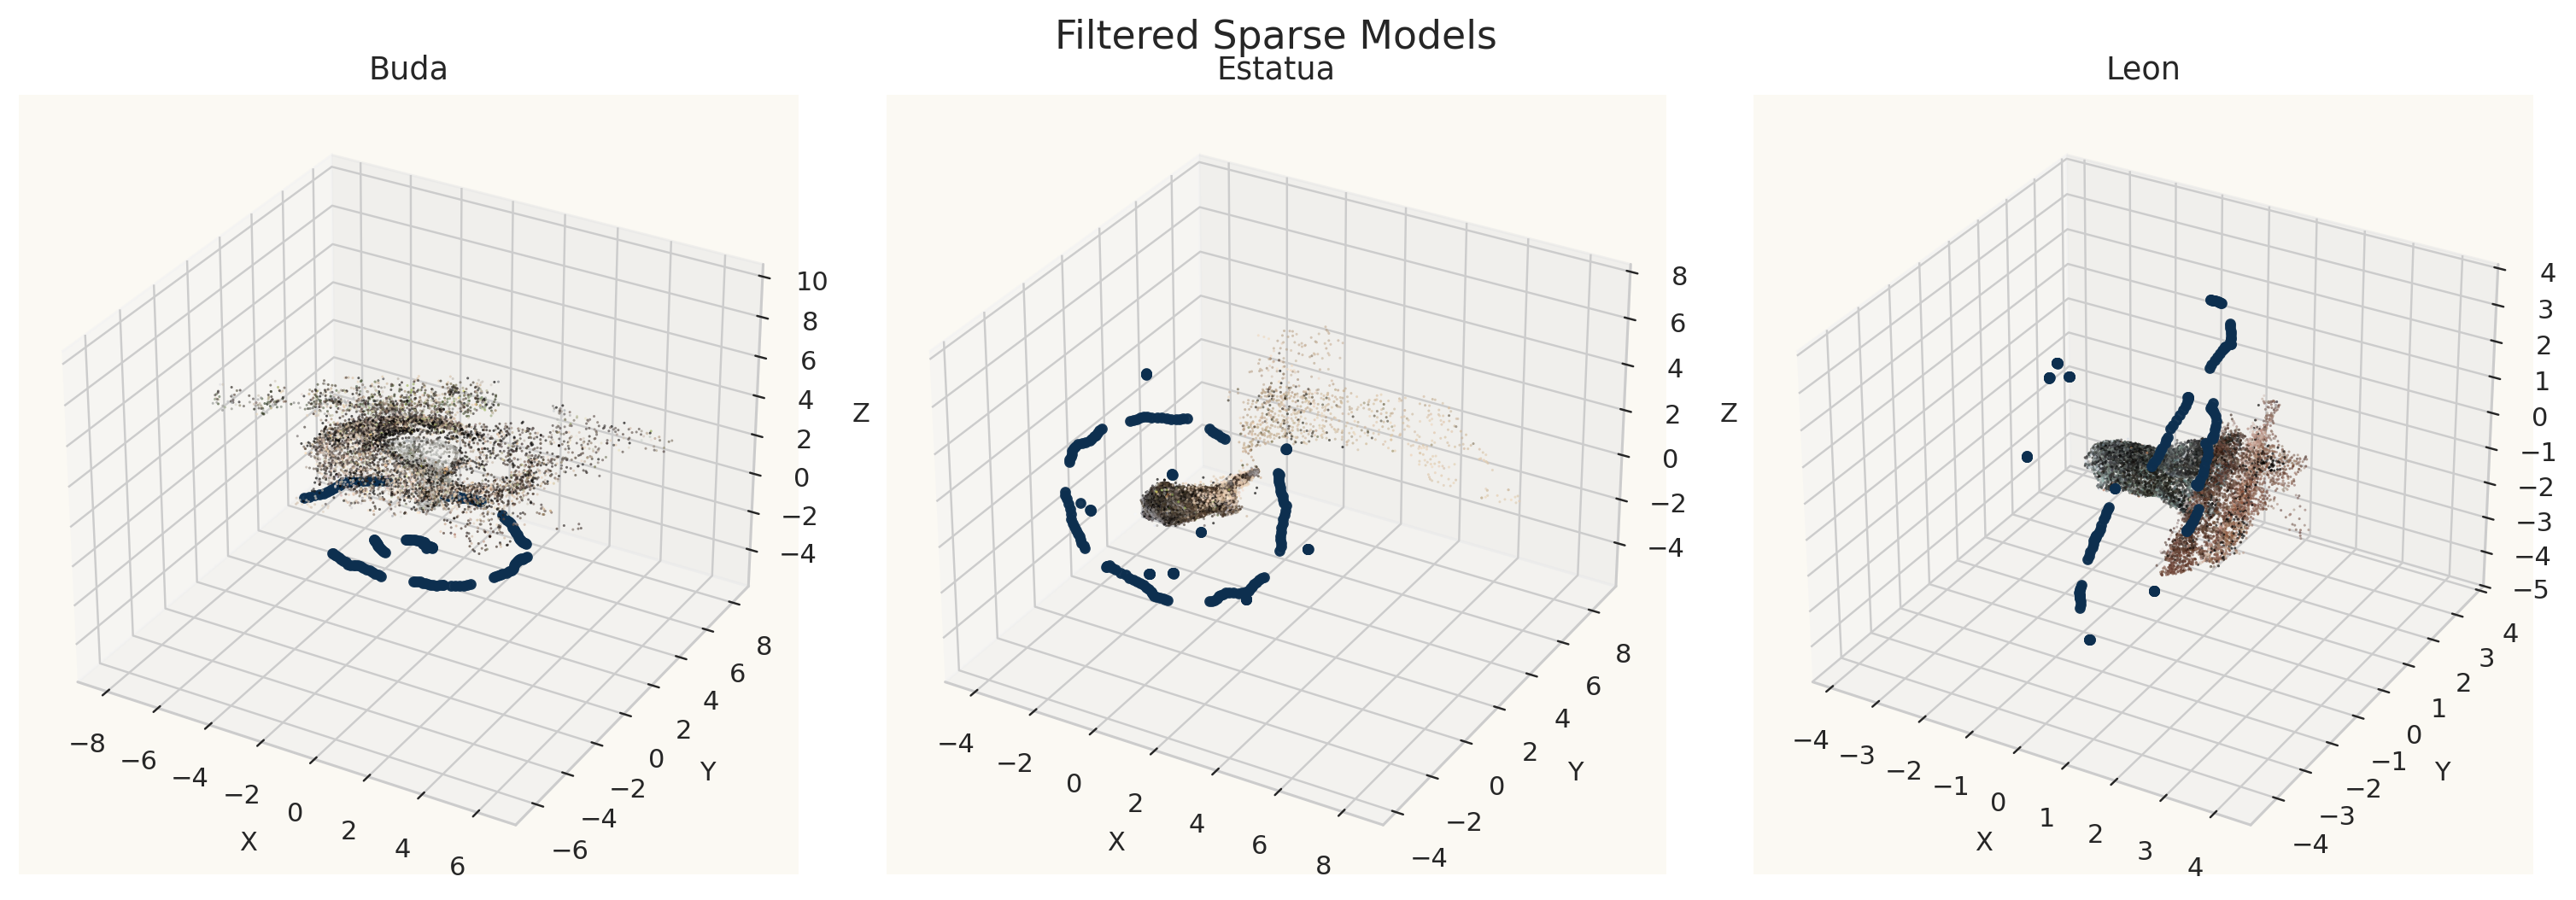
\includegraphics[width=0.95\textwidth]{filtered_pointclouds.png}
  \caption{Modelos dispersos filtrados y centros de c\'amara estimados para los tres objetos.}
  \label{fig:pointclouds}
\end{figure*}

\subsection{Efecto \emph{Doppelganger}}

La consigna pidi\'o inducir deliberadamente el efecto \emph{doppelganger}. En este proyecto se cumpli\'o ejecutando una b\'usqueda exhaustiva auxiliar sobre cada dataset. Los 20 candidatos con mayor puntuaci\'on fueron almacenados por objeto.

La Tabla~\ref{tab:doppel} resume el candidato principal en cada escena. \emph{Buda} muestra los casos m\'as fuertes, con m\'as de 2300 matches crudos y una relaci\'on geom\'etrica cercana a 0.84. Esto indica que las vistas son muy parecidas a nivel visual, pero no completamente equivalentes desde la geometr\'ia epipolar. \emph{Estatua} y \emph{leon} presentan el mismo fen\'omeno, aunque con menos matches.

\begin{table}[htbp]
\caption{Candidato principal de doppelganger por dataset.}
\label{tab:doppel}
\centering
\small
\begin{tabular}{p{1.0cm}p{1.3cm}p{1.0cm}p{0.8cm}p{0.8cm}}
\toprule
\textbf{Obj.} & \textbf{Par} & \textbf{Matches} & \textbf{Geom.} & \textbf{Score} \\
\midrule
Buda & 020-100 & 2563 & 0.833 & 428 \\
Est. & 016-072 & 342  & 0.772 & 78 \\
Leon & 024-026 & 191  & 0.764 & 45 \\
\bottomrule
\end{tabular}
\end{table}

\begin{figure*}[htbp]
  \centering
  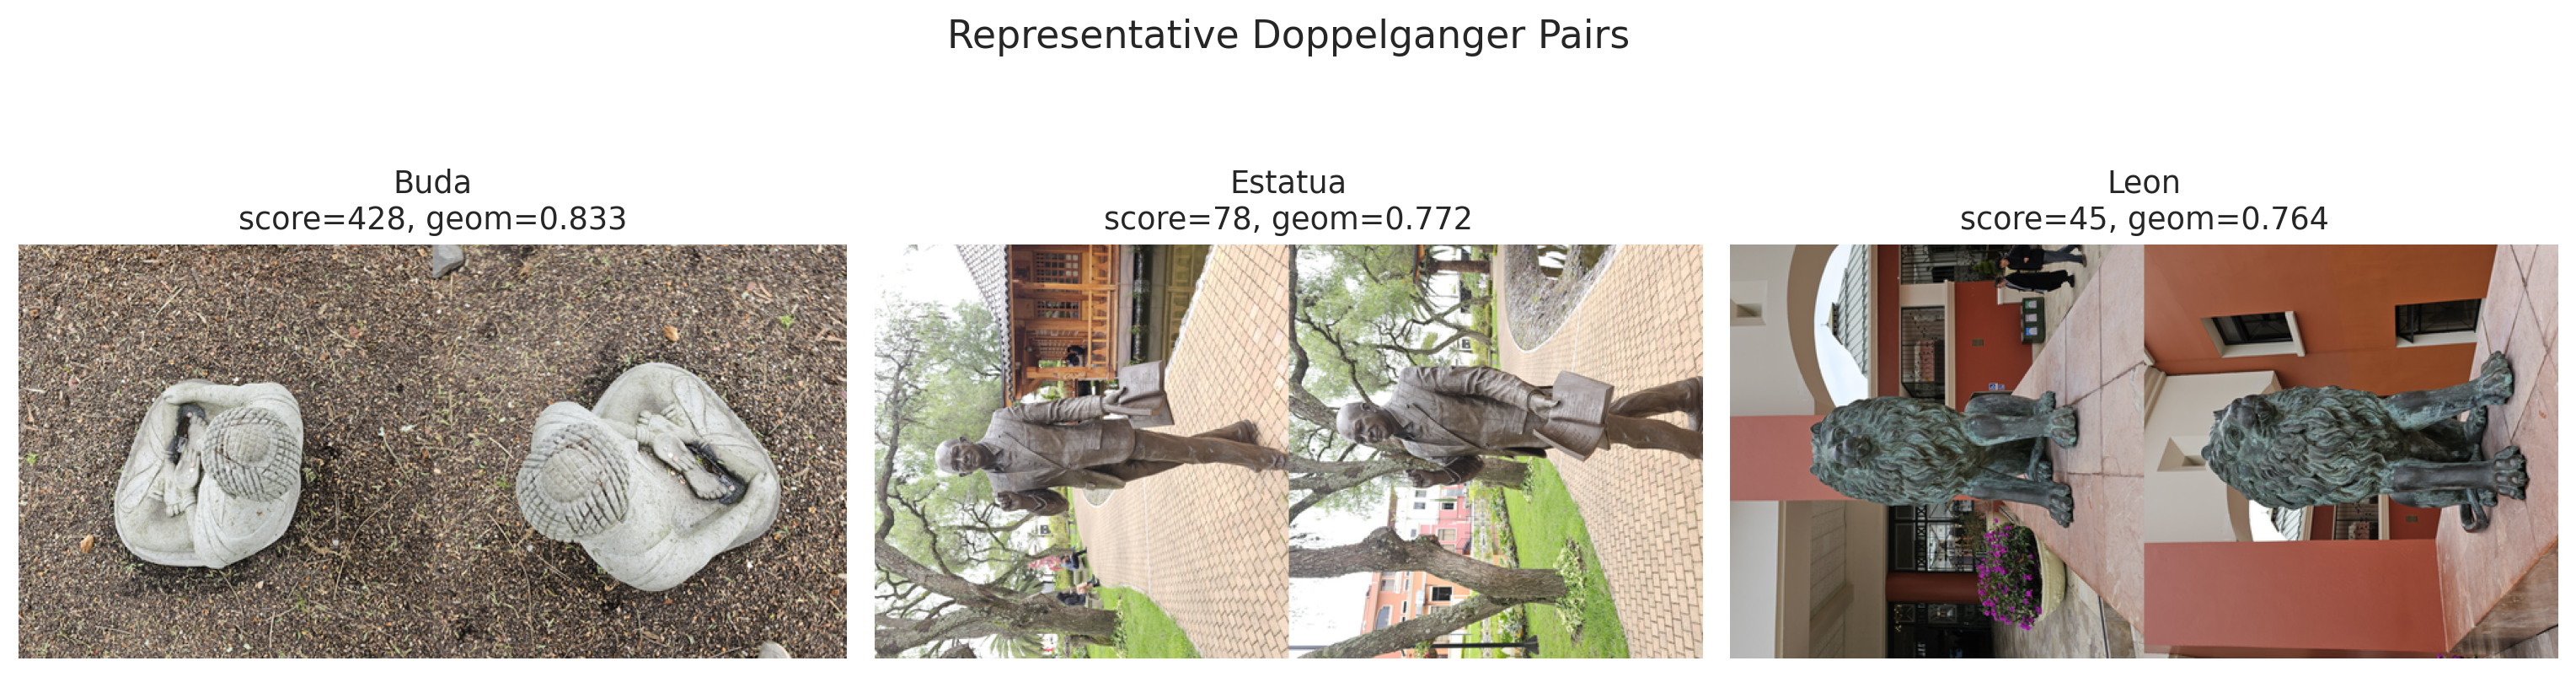
\includegraphics[width=0.95\textwidth]{doppelganger_examples.png}
  \caption{Ejemplos de pares doppelganger detectados autom\'aticamente en los tres objetos.}
  \label{fig:doppel}
\end{figure*}

\section{Discusi\'on}\label{sec:discussion}

Los resultados permiten extraer varias observaciones relevantes.

Primero, la calidad de la captura tiene un efecto directo en la robustez del pipeline. \emph{Buda} y \emph{leon} muestran recorridos m\'as consistentes, lo que se traduce en registro completo y grafos de alta cohesi\'on. En cambio, \emph{estatua} necesita m\'as im\'agenes para estabilizar la reconstrucci\'on y aun as\'i no logra registrar el 100\% del conjunto.

Segundo, el an\'alisis incremental cumple una funci\'on doble: sirve como evidencia acad\'emica del crecimiento del modelo y tambi\'en como herramienta de diagn\'ostico. Por ejemplo, el salto de \emph{leon} entre 40 y 80 im\'agenes revela un umbral pr\'actico de vistas necesarias para cerrar el objeto con suficiente conectividad.

Tercero, el filtrado de nube dispersa no debe verse como un paso cosm\'etico. En este proyecto ayud\'o a remover puntos menos confiables y a enfatizar la geometr\'ia del objeto, mejorando adem\'as ligeramente el error medio de reproyecci\'on.

Finalmente, la adaptaci\'on de un pipeline de producci\'on a un notebook explicativo result\'o valiosa. La reconstrucci\'on completa sobre cientos de im\'agenes es m\'as adecuada para CLI y Docker, mientras que la narrativa por fases, los gr\'aficos y la inspecci\'on de casos doppelganger se benefician de un entorno tipo notebook. De esta forma se concili\'o reproducibilidad con claridad pedag\'ogica.

\section{Conclusiones}\label{sec:conc}

Se implement\'o y document\'o un flujo completo de Structure from Motion para reconstrucci\'on 3D usando tres datasets reales capturados por el equipo. El trabajo no se limit\'o a reconstruir una escena, sino que integr\'o an\'alisis del grafo de vistas, evaluaci\'on incremental, filtrado del modelo y detecci\'on del efecto \emph{doppelganger}.

Las principales conclusiones son:
\begin{enumerate}
  \item el pipeline basado en COLMAP y orquestado desde Python permite reconstrucciones dispersas robustas sobre conjuntos grandes de im\'agenes;
  \item la escena \emph{buda} fue la m\'as estable desde el inicio, mientras que \emph{estatua} represent\'o el caso m\'as desafiante;
  \item \emph{leon} obtuvo la mejor evidencia de estabilidad multi-vista, con registro total y la mayor longitud media de \emph{track};
  \item el filtrado del modelo mejora la interpretabilidad de la nube dispersa y reduce ligeramente el error medio de reproyecci\'on;
  \item el efecto \emph{doppelganger} pudo inducirse y analizarse de forma expl\'icita usando un matching exhaustivo auxiliar;
  \item el notebook de visualizaci\'on complementa de manera natural al pipeline reproducible y cumple mejor con el formato de presentaci\'on exigido por la consigna original.
\end{enumerate}

Como trabajo futuro, se podr\'ia extender el pipeline hacia reconstrucci\'on densa y texturizado, incorporar evaluaci\'on m\'as fina por segmentos del recorrido, y automatizar la exportaci\'on de figuras y tablas directamente desde el notebook hacia el informe.

\begin{thebibliography}{00}
\bibitem{b1} R.~Szeliski, \emph{Computer Vision: Algorithms and Applications}, 2nd ed. Springer, 2022.
\bibitem{b2} J.~L.~Schonberger and J.-M.~Frahm, ``Structure-from-motion revisited,'' in \emph{Proc.\ IEEE CVPR}, 2016, pp.~4104--4113.
\bibitem{b3} J.~L.~Schonberger, E.~Zheng, M.~Pollefeys, and J.-M.~Frahm, ``Pixelwise view selection for unstructured multi-view stereo,'' in \emph{Proc.\ ECCV}, 2016, pp.~501--518.
\bibitem{b4} D.~G.~Lowe, ``Distinctive image features from scale-invariant keypoints,'' \emph{Int.\ J.\ Comput.\ Vis.}, vol.~60, no.~2, pp.~91--110, 2004.
\bibitem{b5} R.~Hartley and A.~Zisserman, \emph{Multiple View Geometry in Computer Vision}, 2nd ed. Cambridge University Press, 2004.
\bibitem{b6} M.~A.~Fischler and R.~C.~Bolles, ``Random sample consensus: A paradigm for model fitting with applications to image analysis and automated cartography,'' \emph{Commun.\ ACM}, vol.~24, no.~6, pp.~381--395, 1981.
\bibitem{b7} S.~Agarwal, N.~Snavely, I.~Simon, S.~M.~Seitz, and R.~Szeliski, ``Building Rome in a day,'' in \emph{Proc.\ IEEE ICCV}, 2009, pp.~72--79.
\end{thebibliography}

\end{document}
